\begin{figure}[H]
\caption{ETL and ELT}
\centering
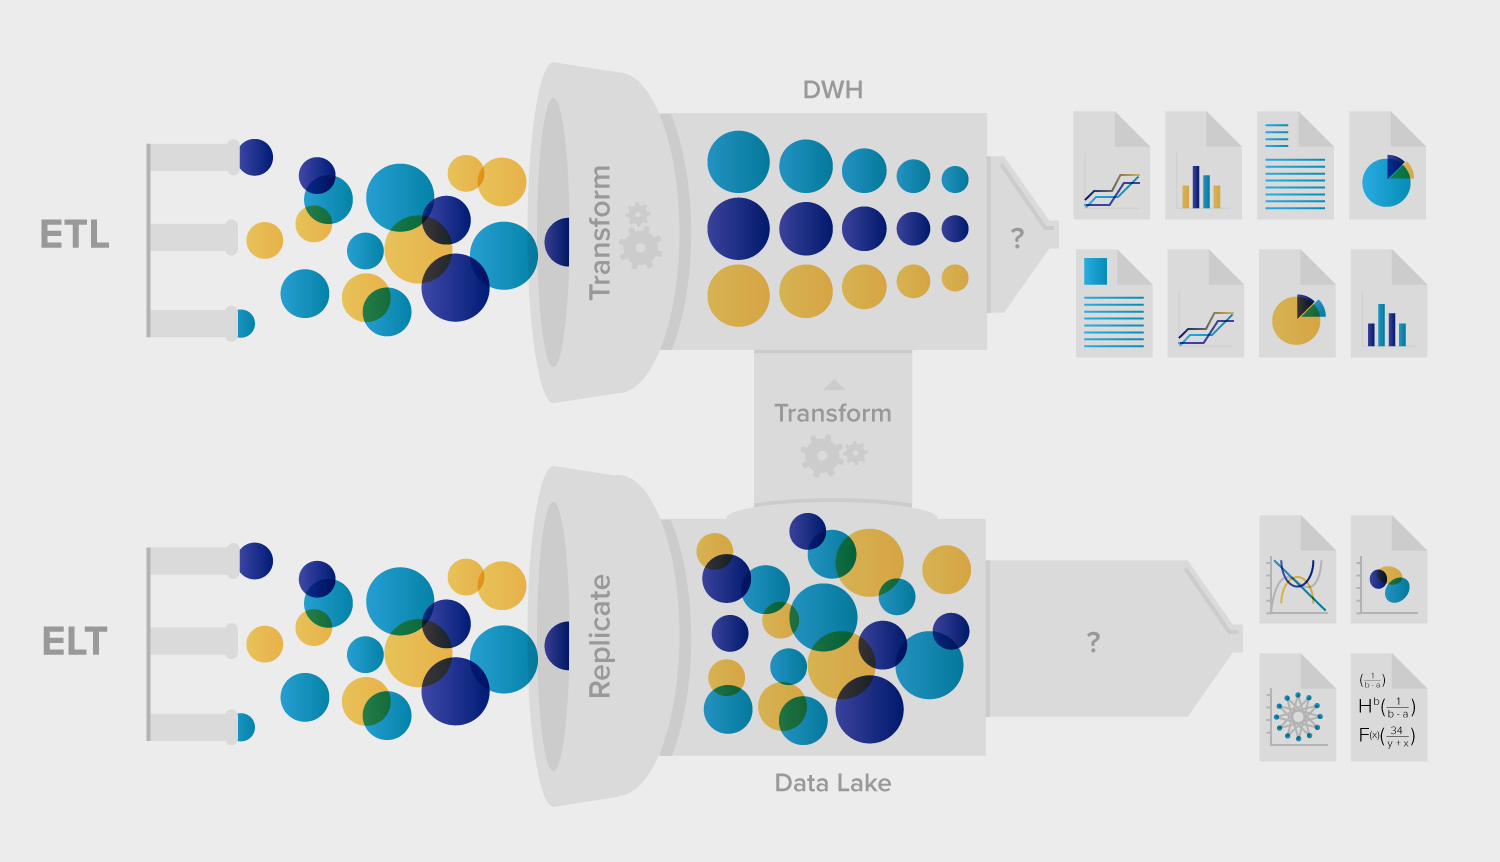
\includegraphics[width=1\linewidth]{images/ETL-ELT.png}
\small
\textit{Note.} The image depicts a comparison between two data processing approaches. ETL (Extract, Transform, Load) and ELT (Extract, Load, Transform). Both processes start with diverse data sources represented by colored circles; ETL transforms data before loading into a data warehouse (DWH); ELT loads data into a data lake first, then transforms it; The outcomes of both processes are visualized as various types of reports and charts
\textit{Creator:} (\cite{etleltDatacamp})\footnote[22]{\fullcite{etleltDatacamp}}
\end{figure}